\chapter[Pre-processing of data]{Pre-processing of stock market and industrial data}
\section{Introduction}
This chapter will introduce the sources of economy data and stock data and the methods to pre-process these data in order to transform and normalise raw data for the further visualisation, construction of networks and topological analysis.

\section{Data source}
This thesis considers 1,418 stocks of listing US companies that were traded consecutively in the NYSE and NASDAQ stock market of US on the trading days from January 4, 2016 to December 30, 2016 and uses daily closing price during this period and the economical use table data from the Industry Economic Accounts (IEAs) of year 2016 in a summary-level of industrial sectors are collected from the official website of Bureau of Economic Analysis, US Department of Commerce \cite{bea}.

\section{Economic Input-Output table}

\begin{figure}
	\begin{center}
		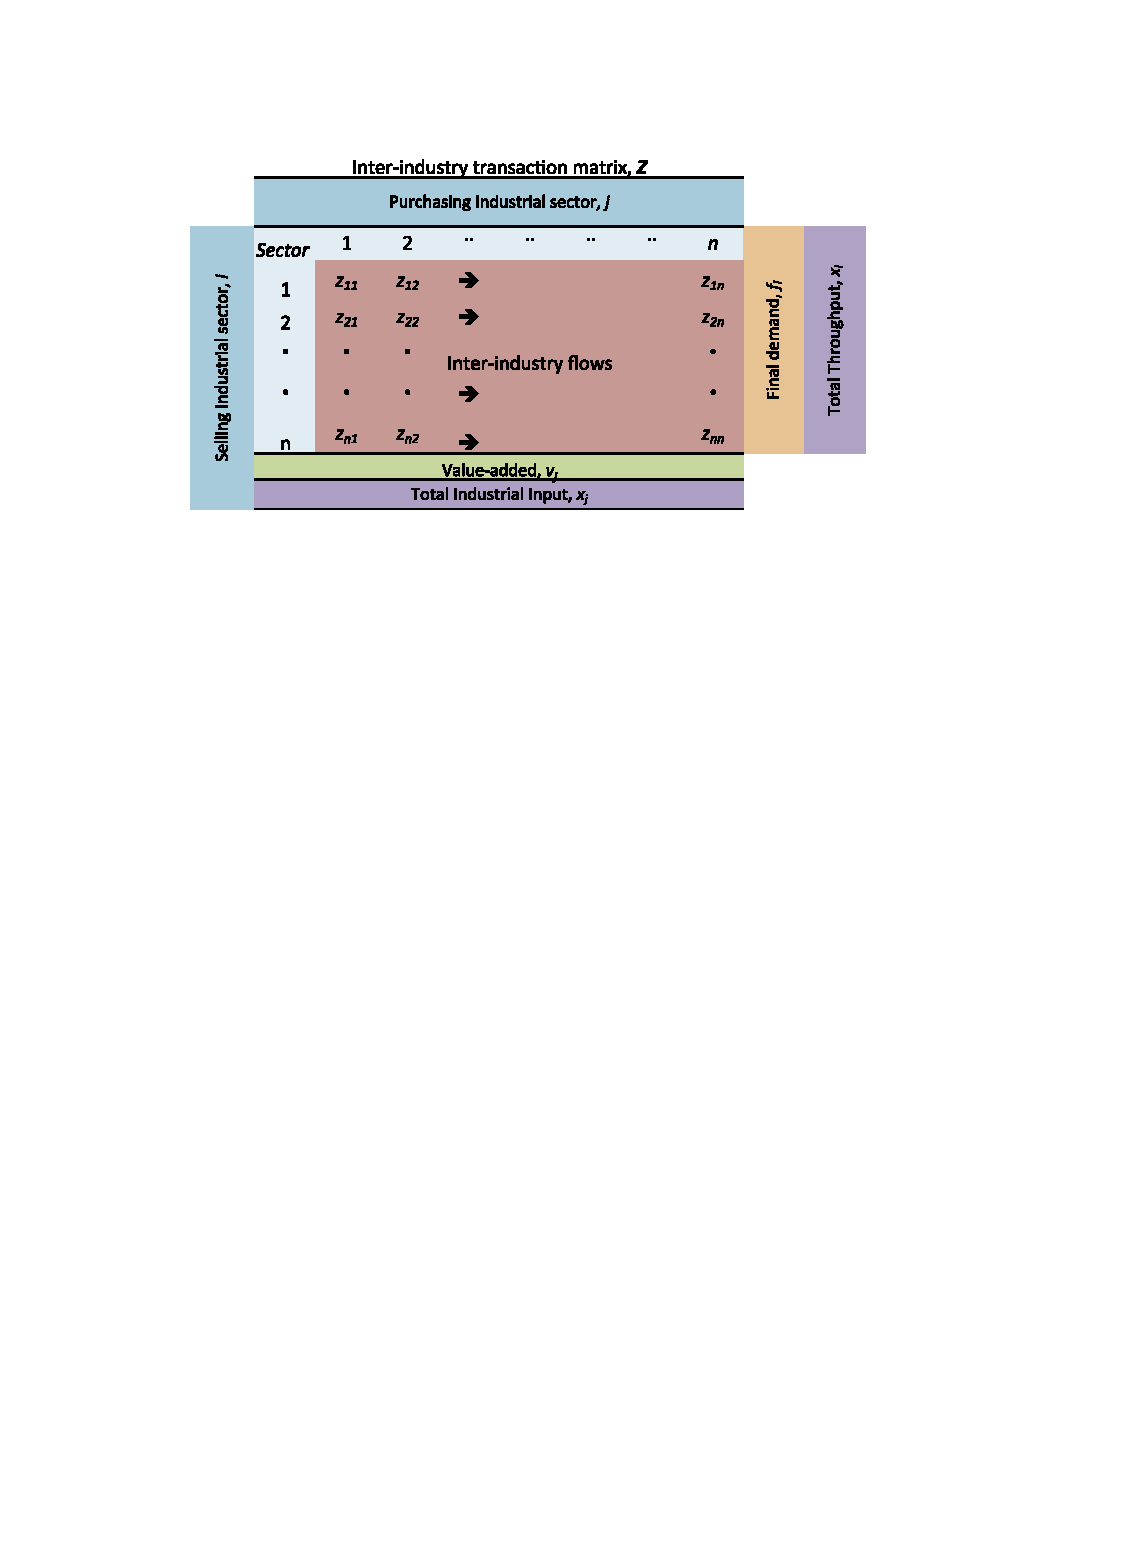
\includegraphics[width=14cm]{EIO_model}
	\end{center}
	\caption{Tabular representation of the Economic Input–Output (EIO) model \cite{CHOPRA2015865}.}
	\label{fig:EIO_model}
\end{figure}

The Bureau of Economic Analysis (BEA) in the US publishes Economic Input-Output (EIO) tables each year, which are the transaction matrices of all purchases and sales between sectors in a certain industry group level of a year, i.e. depict how industries provide input to, and use output from, each other to produce Gross Domestic Product (GDP). The tabular representation of EIO model is illustrated in the figure \ref{fig:EIO_model}.

This thesis uses the use table of 2016 corresponding to the same year of the studied stock market. As the figure \ref{fig:EIO_model} shows, among the transaction matrix \textbf{Z} there are Total Industry Input row \textbf{I} at the bottom and the Total Industry Output column \textbf{O} at the right are the statistics of total purchase by each sectors and total sales from each sectors respectively. The elements of the normalised direct demand matrix \textbf{A} and the direct requirement matrix \textbf{B} are:

\begin{eqnarray}\label{equ:eio_i}
a_{i,j} = -log_{10}{\frac{z_{i,j}}{I_j N_j}}^{-1}
\end{eqnarray}

and

\begin{eqnarray}\label{equ:eio_o}
b_{i,j} = -log_{10}{\frac{z_{i,j}}{O_i N_i}}^{-1}
\end{eqnarray}

respectively. $N_i$ is the number of stocks in the industrial sector which stock $i$ belongs to. Moreover, certain threshold values $\theta_{DD}$ and $\theta_{DR}$ are specified and a directed edge can be added between stock $i$ and stock $j$ if the value of $a_{i,j}$ is greater than $\theta_{DD}$ or the value of $c_{i,j}$ is greater than $\theta_{DR}$.

Understanding patterns of connections in the stock networks is essential, while using the EIO table as a part of networks permits analysis of network topological properties by the approaches of statistics and complex networks theory from the views of economical fundamentals (EIO table) and technical indicators (correlation coefficient, as will be introduced below).

\section{Logarithmic return of stock prices}
Using stock price returns, instead of stock prices, can allow us to measure all variables in a comparable metric, therefore enabling evaluation of analytic relationships amongst two or more variables despite originating from price series of unequal values.

Logarithmic return of a stock in this thesis is calculated as the log of the close price of one day divided by the close price of the previous day, which is obtained from the following formula:
\begin{eqnarray}\label{equ:log}
r_i(\tau)=lnP_i(\tau)-lnP_i(\tau-\Delta t)
\end{eqnarray}

The critical properties of logarithmic stock price returns which are useful for the research are listed below :
\begin{itemize}
	\item Log-normality: if we assume that prices are distributed log normally, then $log(1 + r_i)$ is conveniently normally distributed.
	\item Approximate raw-log equality: when returns are very small, it can ensure that the logarithmic returns are close in value to the raw returns.
	\item Time-additivity: the compound raw return over $n$ periods is merely the difference in log between initial and final periods.
\end{itemize}

In a nutshell, as a proxy for the percentage change in the price, logarithmic return is symmetric and has mathematical conveniences for adding up or subtracting values on the log scale, which are useful for mathematical finance. Therefore, logarithmic return is used as the measure of price changes in this thesis.

\section{Correlation coefficient}
Correlation coefficient, short for Pearson correlation coefficient \cite{pearson1895note}, is a measure of the linear correlation between two variables X and Y, the value of which is in the range of $\left[-1,1\right]$, where $1$ means total positive linear correlation, $0$ means no linear correlation, and $-1$ means total negative linear correlation. It is widely used in the quantitative finance. 

Correlation coefficient between two stocks is considered in terms of the matrix \textbf{C}, as the following equation shows:
\begin{eqnarray}\label{equ:corr}
c_{i,j}=\frac{\langle r_ir_j \rangle-\langle r_i\rangle \langle r_j\rangle}{\sqrt{(\langle r_i^2\rangle-\langle r_i\rangle^2)(\langle r_j^2\rangle-\langle r_j\rangle^2)}}
\end{eqnarray}

where $r$ denotes the return and the bracket indicates a temporal average over the period. Additionally, a certain threshold value $\theta_{corr}$, $0\leq \theta_{corr} \leq1$ is specified, and a directed edge is qualified to be linked between stock $i$ and stock $j$ if the value of $c_{i,j}$ is greater than or equal to $\theta_{corr}$.

\section{Summary}
In this chapter the data sources together with the pre-processing methods have been introduced. Hence, the table of economical data are converted into matrix and the stock price data are transformed to logarithmic return data and correlation coefficients for further analysis.